\documentclass[twocolumn]{article}
\usepackage{graphicx}
\usepackage{amsmath}
\usepackage{float}
\usepackage{algpseudocode}
\usepackage{url}
\usepackage{amssymb}
\usepackage{bbm}
\renewcommand{\algorithmicforall}{\textbf{for each}}
\usepackage{tikz}
\usepackage{dsfont}
\providecommand{\abs}[1]{\lvert#1\rvert}
\providecommand{\Abs}[1]{\bigg\lvert#1\bigg\rvert}
\providecommand{\norm}[1]{\lVert#1\rVert}
\providecommand{\ceil}[1]{\lceil#1\rceil}
\usetikzlibrary{arrows}
\usepackage[margin=0.7in]{geometry}

\begin{document}

\author{
  Bryan McCann\\
  Stanford University\\
  \texttt{bmccann@stanford.edu}
  \and
 Zachary Yellin-Flaherty\\
  Stanford University\\
  \texttt{zachyf@stanford.edu}
}
\title{CS 221- Final Report}
\date{}

\maketitle

\section*{Abstract}

\emph{Bach and other Classical-era composers wrote melodies that, when combined with some hidden permutation of the melody riddle, yield beautiful contrapuntal canons.  In this paper, we outline a method for modeling musical fluency and use that model to solve some of Bach's riddles.}

\section{Introduction}

We set out to design a system that can solve the Puzzle Canons posed by Bach. Canons typically consist of one single-voiced melody that can be transformed in an enumerable set ways to create a poly-textural musical piece that follows all the conventions of classical harmonic practices. It is common to call the proposed melody the theme, and the transformations variations on the theme. Classical composers would sometimes challenge each other with these puzzle canons, and some remain unsolved. \\

\begin{figure}[H]
    \centering
    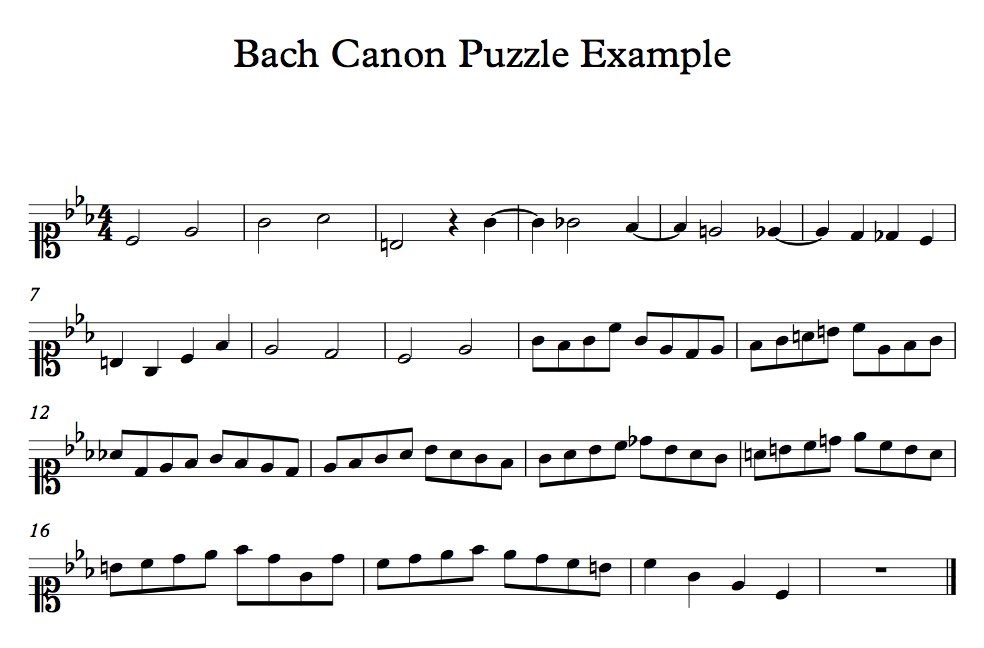
\includegraphics[width=0.5\textwidth]{theme.png}
    \caption{The Cancrizans}
    \label{fig:awesome_image}
\end{figure}

On a high level, our method consists of two steps:
\begin{enumerate}
\item
Construct a model of musical �fluency� primarily based on harmonic principles.
\item
Frame the search for solutions to Bach�s canons as a search problem with costs determined by our Musical Fluency Model. Then use Uniform Cost Search to solve.
\end{enumerate}



\section{Data Collection and Handling}

We used an MIT python library, music21, which abstracts away virtually all of the technical music aspects of our data. music21 comes with a corpus of music, which includes 148 Bach chorales, which were used to train the Musical Fluency Model described below. 

\section{Baseline Testing}

In our baseline testing we framed the problem as a search problem and used uniform cost search to construct a simple two-part round.  We represented the song �Row, Row, Row Your Boat�, and then asked our algorithm to define the best second voice based on the costs of consonance and dissonance.  The result, which is included in the supplementary materials, is quite harmonic.  While it didn�t assign the highest score to the second voice that we sang in elementary school, the result it chose was the most harmonic in terms of the attributes we gave it.  
2
We simplified our problem statement and model for baseline testing by using a smaller set of actions (only time-shifting) and using a simplified state (pitch, duration).

Notably, the simple song we chose has more options for harmonious voices than more melodically complex pieces.  Since all notes are diationic to the major key (in our case C major), many of the choices scored in a similar range.  With more complex melodies, including Bach�s puzzles tackled by methods described in the next two sections, unintended melodies become more blatantly incorrect, and they yield fewer acceptable outputs.  In fact, part of the criteria in Bach�s time of creating a canon puzzle is that only the correct answer sounds consonant, and as a result the correct answer is obvious when achieved. 

\section{Modeling Harmonic Style}

Several important questions arise when modeling these musical puzzles. How does one train with Bach chorales? How should music be represented as features? Which features determine solutions to Puzzle Canons? What is a reasonable interpretation of musical fluency? 

Two major insights allowed us to simplify the problem and provide modeled solutions to questions we faced. 
\begin{enumerate}
\item Since we are solving Bach�s Puzzle Canons, we only need musical data that represents Bach�s musical style well enough to solve his problems the way that he would have done it.
\item The canons were based on a strict contrapuntal style, and thus we based our model on the assumption that Bach would have made solutions harmonically superior to other proposed solutions.
\end{enumerate}

These insights greatly simplified the modeling process. Musical fluency translates to �most harmonic�, and the standard for �most harmonic� is Bach�s harmonic style. We can abstract away notes and only consider chords and intervals as only they contribute to harmony. Use a bag of chords and intervals to treat harmonic style just as we would linguistic style, creating a vector phi(x). Use the Bach chorale data to find a vector B of average frequencies of the N-grams, which becomes our standard of musical fluency.

\subsection{Model Construction}

In order to construct our model, we extract bigram, trigram, and tetragram features from our corpus of Bach chorales. This process is analogous to extracting features in natural language processing, but the words in this case are intervals if we have only two voices and chords if there are more than two voices. A bigram would then consist of a tuple $(IntervalA, IntervalB)$ in the case of two voices or $(ChordA, ChordB)$ in the case of more than two voices. 

\begin{figure}[H]
    \centering
    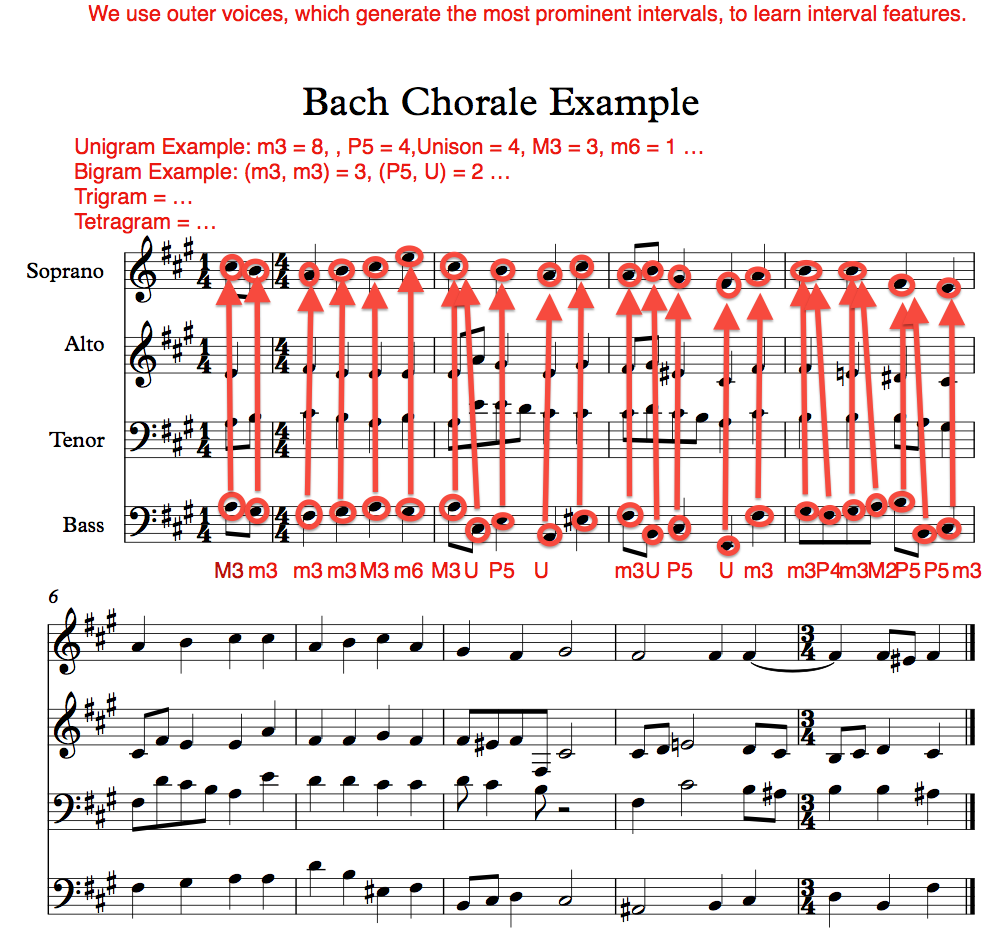
\includegraphics[width=0.4\textwidth]{chorale.png}
    \caption{Chorale Interval Features}
    \label{fig:awesome_image1}
\end{figure}

Because our model is primarily concerned with harmony, we abstract away the notes of the intervals and chords. We consider only the Roman numeral assignments of the chords determined by the current key and the chromatic intervals between the outer voices for two-part harmony. For example, our bigram features might look like $(I, ii6), (ii6, V), (V, I)$. This feature vector would show that the analyzed music contained the common I-ii - V I progression in a major key to begin the piece, with the ii chord in first inversion. The analyzed music might have been CMajor, dminor/F, GMajor, CMajor, but our model ignores those specifics.  In order to accomplish this abstraction, we leveraged Music21�s ability to generate a Roman numeral analysis and interval analysis given a score with multiple voices.  

\begin{figure}[H]
    \centering
    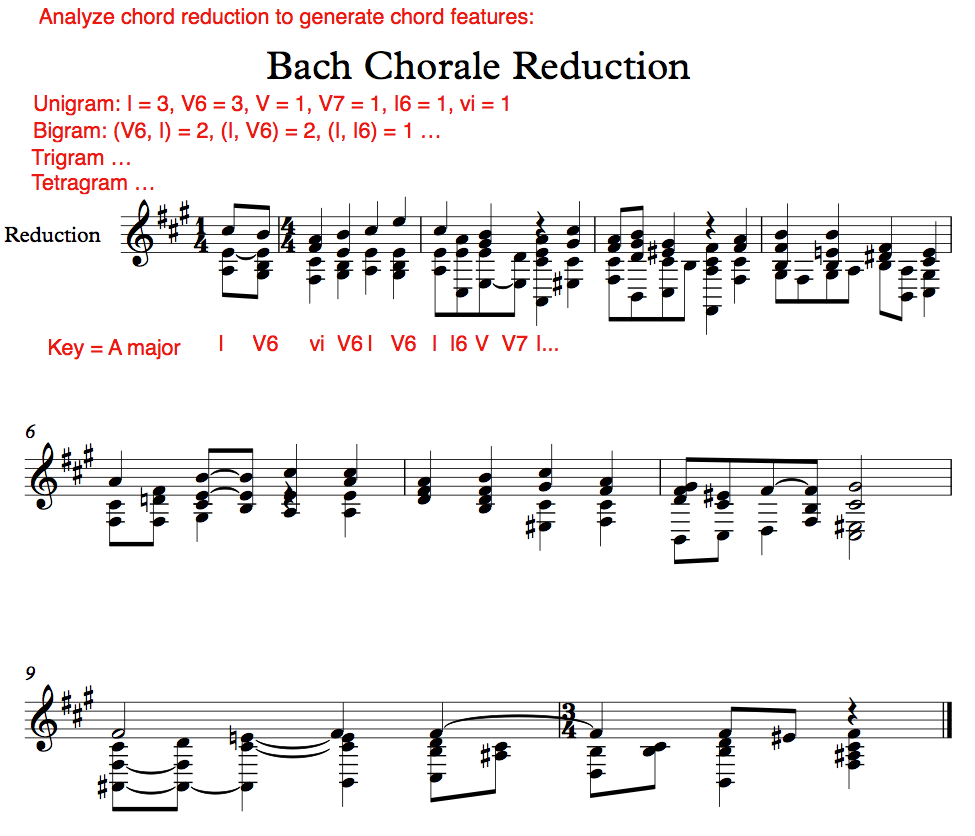
\includegraphics[width=0.4\textwidth]{chorale_reduction.png}
    \caption{Chorale Chord Features}
    \label{fig:awesome_image2}
\end{figure}

\subsection{Rationale}
Modeling only the relationships between chords and intervals allows us to learn how Bach constructs harmonic progressions . We do not include unigrams because this too would give too much information irrelevant to the harmony of the pieces. Bigrams allow the model to capture relationships from one chord to the next, and trigrams and tetragrams capture chord progressions. The model considers fluency as primarily grounded in the frequency of these chord and interval N-grams. For example, in the large corpus that we analyzed, Bach used some bigrams upwards of 25 times, whereas most bigrams present only occur once. The model then suggests that these bigrams are preferred over others in musical and harmonic fluency when they are valid options. 

\subsection{Application}
Our model can be viewed in two ways. First, it is a model of harmonic fluency based on frequency, but it is also intended to serve as a cost function.

 The function is simple. Consider $x$ to be our musical piece, let $\phi(x)$ be our vector of extracted chord/interval features, and let $\beta$ be our vector of chord/interval features extracted from Bach chorales where the values of each entry correspond to the average frequency of that feature in the selection from which it was drawn. So in the case of $x$, an entry in $\phi(x)$ will correspond to the number of times that N-gram appeared in $x$. In the case of $\beta$, an entry will be the average number of times that feature appeared in the corpus of Bach chorales. Then the cost for that $x$ will be the Euclidean distance from $\phi(x)$ to $B$. This will allow our model to suggest that adhering to Bach�s averages is a good indicator that you will be both harmonically and stylistically similar to Bach in solving the Puzzle Canons.

\section{Solving the Puzzle Canons: Searching for the Right Answer}

We frame the problem of solving a Puzzle Canon as a search problem, on which we can use Uniform Cost Search. The input to our problem is the theme, a single voice melody that we have preprocessed using the Music21 python libraries. 

The start state is a music21 stream that represents our theme and a Euclidean distance (cost of accepting this state as a solution) of Infinity as the theme itself is not a viable solution. 

The possible actions are $12$ transpositions for each chromatic interval, $n$ imitations (where $n$ is the number of notes in the original melody so we can have $n$ shifts of the melody), and a mirror, or reversal, of the original melody.

The search consists of iterating through all of the  possible variations of the theme,  calculating their cost by using our model of musical fluency, minimizing the cost, and checking whether we are in and end state. 

There is one condition for an end state: the move does not make sufficient progress towards Bach�s averages according to some tolerance.

Since duration of the entire piece is conserved after each of these transformations, each voice will add harmony to our previous state.  As a result, these multiple voices can be reduced to chords or intervals and then analyzed harmonically. Thus, our search problem with a them of $n$ notes, takes the form:

 \begin{center}
 \begin{tabular}{rl}
 $State_{\text{start}}$: & the theme \\
 $Actions$: & $12$ transpositions, \\
 & $n$ imitations, \\
 & and a mirror \\
 $Cost$: & $\|\beta - \phi(x) \|_2$ \\
 $isGoal$:& $\|\beta - \phi(x) \|_2 < \epsilon$
 \end{tabular}
 \end{center}

\section{Conclusion}
\subsection{Results}
Figure 4 shows sample output for the first Puzzle Cannon, a variation on the King�s Royal Theme and puzzle 1 in our supplementary materials.  In general, the  algorithm returns a set of transformations added to the score with the original puzzle. We currently solve only single-voiced themes, two of which are included in the supplementary materials as examples. 
 \begin{figure}[H]
    \centering
    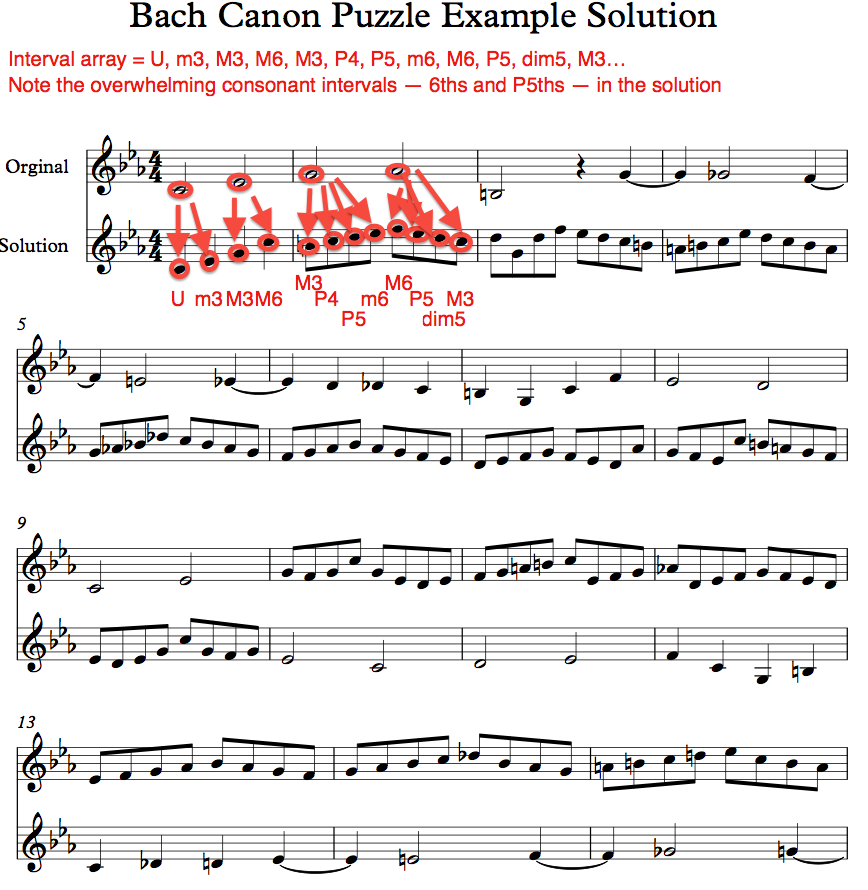
\includegraphics[width=0.4\textwidth]{solution.png}
    \caption{Example Solution}
    \label{fig:awesome_image2}
\end{figure}
\subsection{Takeaway}
After abstracting away music-theory details, modeling music using chord and interval N-grams proved to be effective when combined with a standard of fluency. We gained insight into how to model problems that, at first glance, do not look like search problems, feature extraction problems, and machine learning problems. 
\subsection{Possible Future Work}
In the future, work can be done to deal with Puzzle Canons that start with multiple themes. This blows up the state space exponentially, but its predictability would allow for pruning methods and more advanced systems to tackle these problems.

\end{document}